% Options for packages loaded elsewhere
\PassOptionsToPackage{unicode}{hyperref}
\PassOptionsToPackage{hyphens}{url}
%
\documentclass[
  ignorenonframetext,
  aspectratio=54,
]{beamer}
\usepackage{pgfpages}
\setbeamertemplate{caption}[numbered]
\setbeamertemplate{caption label separator}{: }
\setbeamercolor{caption name}{fg=normal text.fg}
\beamertemplatenavigationsymbolsempty
% Prevent slide breaks in the middle of a paragraph
\widowpenalties 1 10000
\raggedbottom
\setbeamertemplate{part page}{
  \centering
  \begin{beamercolorbox}[sep=16pt,center]{part title}
    \usebeamerfont{part title}\insertpart\par
  \end{beamercolorbox}
}
\setbeamertemplate{section page}{
  \centering
  \begin{beamercolorbox}[sep=12pt,center]{part title}
    \usebeamerfont{section title}\insertsection\par
  \end{beamercolorbox}
}
\setbeamertemplate{subsection page}{
  \centering
  \begin{beamercolorbox}[sep=8pt,center]{part title}
    \usebeamerfont{subsection title}\insertsubsection\par
  \end{beamercolorbox}
}
\AtBeginPart{
  \frame{\partpage}
}
\AtBeginSection{
  \ifbibliography
  \else
    \frame{\sectionpage}
  \fi
}
\AtBeginSubsection{
  \frame{\subsectionpage}
}
\usepackage{lmodern}
\usepackage{amssymb,amsmath}
\usepackage{ifxetex,ifluatex}
\ifnum 0\ifxetex 1\fi\ifluatex 1\fi=0 % if pdftex
  \usepackage[T1]{fontenc}
  \usepackage[utf8]{inputenc}
  \usepackage{textcomp} % provide euro and other symbols
\else % if luatex or xetex
  \usepackage{unicode-math}
  \defaultfontfeatures{Scale=MatchLowercase}
  \defaultfontfeatures[\rmfamily]{Ligatures=TeX,Scale=1}
\fi
% Use upquote if available, for straight quotes in verbatim environments
\IfFileExists{upquote.sty}{\usepackage{upquote}}{}
\IfFileExists{microtype.sty}{% use microtype if available
  \usepackage[]{microtype}
  \UseMicrotypeSet[protrusion]{basicmath} % disable protrusion for tt fonts
}{}
\makeatletter
\@ifundefined{KOMAClassName}{% if non-KOMA class
  \IfFileExists{parskip.sty}{%
    \usepackage{parskip}
  }{% else
    \setlength{\parindent}{0pt}
    \setlength{\parskip}{6pt plus 2pt minus 1pt}}
}{% if KOMA class
  \KOMAoptions{parskip=half}}
\makeatother
\usepackage{xcolor}
\IfFileExists{xurl.sty}{\usepackage{xurl}}{} % add URL line breaks if available
\IfFileExists{bookmark.sty}{\usepackage{bookmark}}{\usepackage{hyperref}}
\hypersetup{
  pdftitle={Pipeline Data Academy},
  pdfauthor={Miklós Koren},
  hidelinks,
  pdfcreator={LaTeX via pandoc}}
\urlstyle{same} % disable monospaced font for URLs
\newif\ifbibliography
\usepackage{graphicx}
\makeatletter
\def\maxwidth{\ifdim\Gin@nat@width>\linewidth\linewidth\else\Gin@nat@width\fi}
\def\maxheight{\ifdim\Gin@nat@height>\textheight\textheight\else\Gin@nat@height\fi}
\makeatother
% Scale images if necessary, so that they will not overflow the page
% margins by default, and it is still possible to overwrite the defaults
% using explicit options in \includegraphics[width, height, ...]{}
\setkeys{Gin}{width=\maxwidth,height=\maxheight,keepaspectratio}
% Set default figure placement to htbp
\makeatletter
\def\fps@figure{htbp}
\makeatother
\setlength{\emergencystretch}{3em} % prevent overfull lines
\providecommand{\tightlist}{%
  \setlength{\itemsep}{0pt}\setlength{\parskip}{0pt}}
\setcounter{secnumdepth}{-\maxdimen} % remove section numbering
\usepackage{pgfpages}
\usepackage{luatexbase}
\usepackage{microtype}
\usepackage{luatextra}
\usepackage{luaotfload}
\usepackage{fontspec}
\usepackage{unicode-math}

\setmainfont[
Extension=.otf,
UprightFont={IBM Plex Serif-Text},
BoldFont={IBM Plex Serif-Bold},
ItalicFont={IBM Plex Serif-Italic},
BoldItalicFont={IBM Plex Serif-BoldItalic}
]{IBM Plex Serif}[Ligatures=TeX,Scale=MatchUppercase]
% Scales Plex to default size, e.g., to Helvetica´s size.

\setmonofont{IBM Plex Mono Text}[Scale=MatchLowercase,
Ligatures=TeX]
\setsansfont{IBM Plex Sans Text}[Scale=MatchUppercase,
Ligatures=TeX]
\setmathfont{Latin Modern Math}

% CEU style guide
% https://www.ceu.edu/sites/default/files/attachment/article/13110/ceugraphicsstandardsguideapril2015.pdf
\definecolor{CTred}{RGB}{229,32,32}
\definecolor{CTgrey}{RGB}{153,153,153}


% colors: white text on 90% black background
\setbeamercolor{normal text}{fg=black,bg=white}

% light blue as a highlight color
\setbeamercolor*{structure}{fg=CTred}
\setbeamercolor{section title}{fg=CTred}
\setbeamercolor{alerted text}{use=structure,fg=CTred}
\setbeamercolor*{palette primary}{use=structure,fg=structure.fg}
\setbeamercolor*{palette secondary}{use=structure,fg=structure.fg!95!black}
\setbeamercolor*{palette tertiary}{use=structure,fg=structure.fg!90!black}
\setbeamercolor*{palette quaternary}{use=structure,fg=structure.fg!95!black,bg=black!80}

\setbeamercolor*{framesubtitle}{fg=white}


% use system fonts: here, Gill Sans
\usefonttheme{professionalfonts}
\setbeamerfont{quote}{shape=\upshape}

% eliminate silly beamer navigation line at bottom of slides
\setbeamertemplate{navigation symbols}{}

% ensure text jusfication
\usepackage{ragged2e}
\justifying

% pandoc makes 2nd-lever headers into blocks, and this ensures justification
% in blocks too
\addtobeamertemplate{block begin}{}{\justifying}




\urlstyle{same}
\usepackage[overlay,absolute]{textpos}

\setbeamertemplate{itemize items}[square]

\TPGrid[10 mm,8 mm]{9}{8}
% beamer's left and right margin is 10 mm. The top/bottom margin is ??
% or without a header ??
% the slide dimensions are 128 mm x 96 mm
% so the resulting \TPHorizModule = 12 mm and \TPVertModule = 10 mm

% uncomment if you want biblatex for citations on slides

% \usepackage{csquotes}
% \usepackage[notes,short,noibid,backend=biber]{biblatex-chicago}
% \bibliography{course.bib} 

\titlegraphic{
\includegraphics[width=0.33\paperwidth]{../assets/logo/Horizontal/RGB/pdf/Koren_logo_horizontal_RGB_colorful.pdf}}
\providecommand{\exhibit}[2]{\includegraphics[keepaspectratio, height=0.9\textheight, width=\textwidth]{assets/img/#1}\\ {\tiny #2}}

\title{Pipeline Data Academy}
\author{Miklós Koren}
\date{}

\begin{document}
\frame{\titlepage}

\hypertarget{introduction}{%
\section{Introduction}\label{introduction}}

\begin{frame}{My first program}
\protect\hypertarget{my-first-program}{}
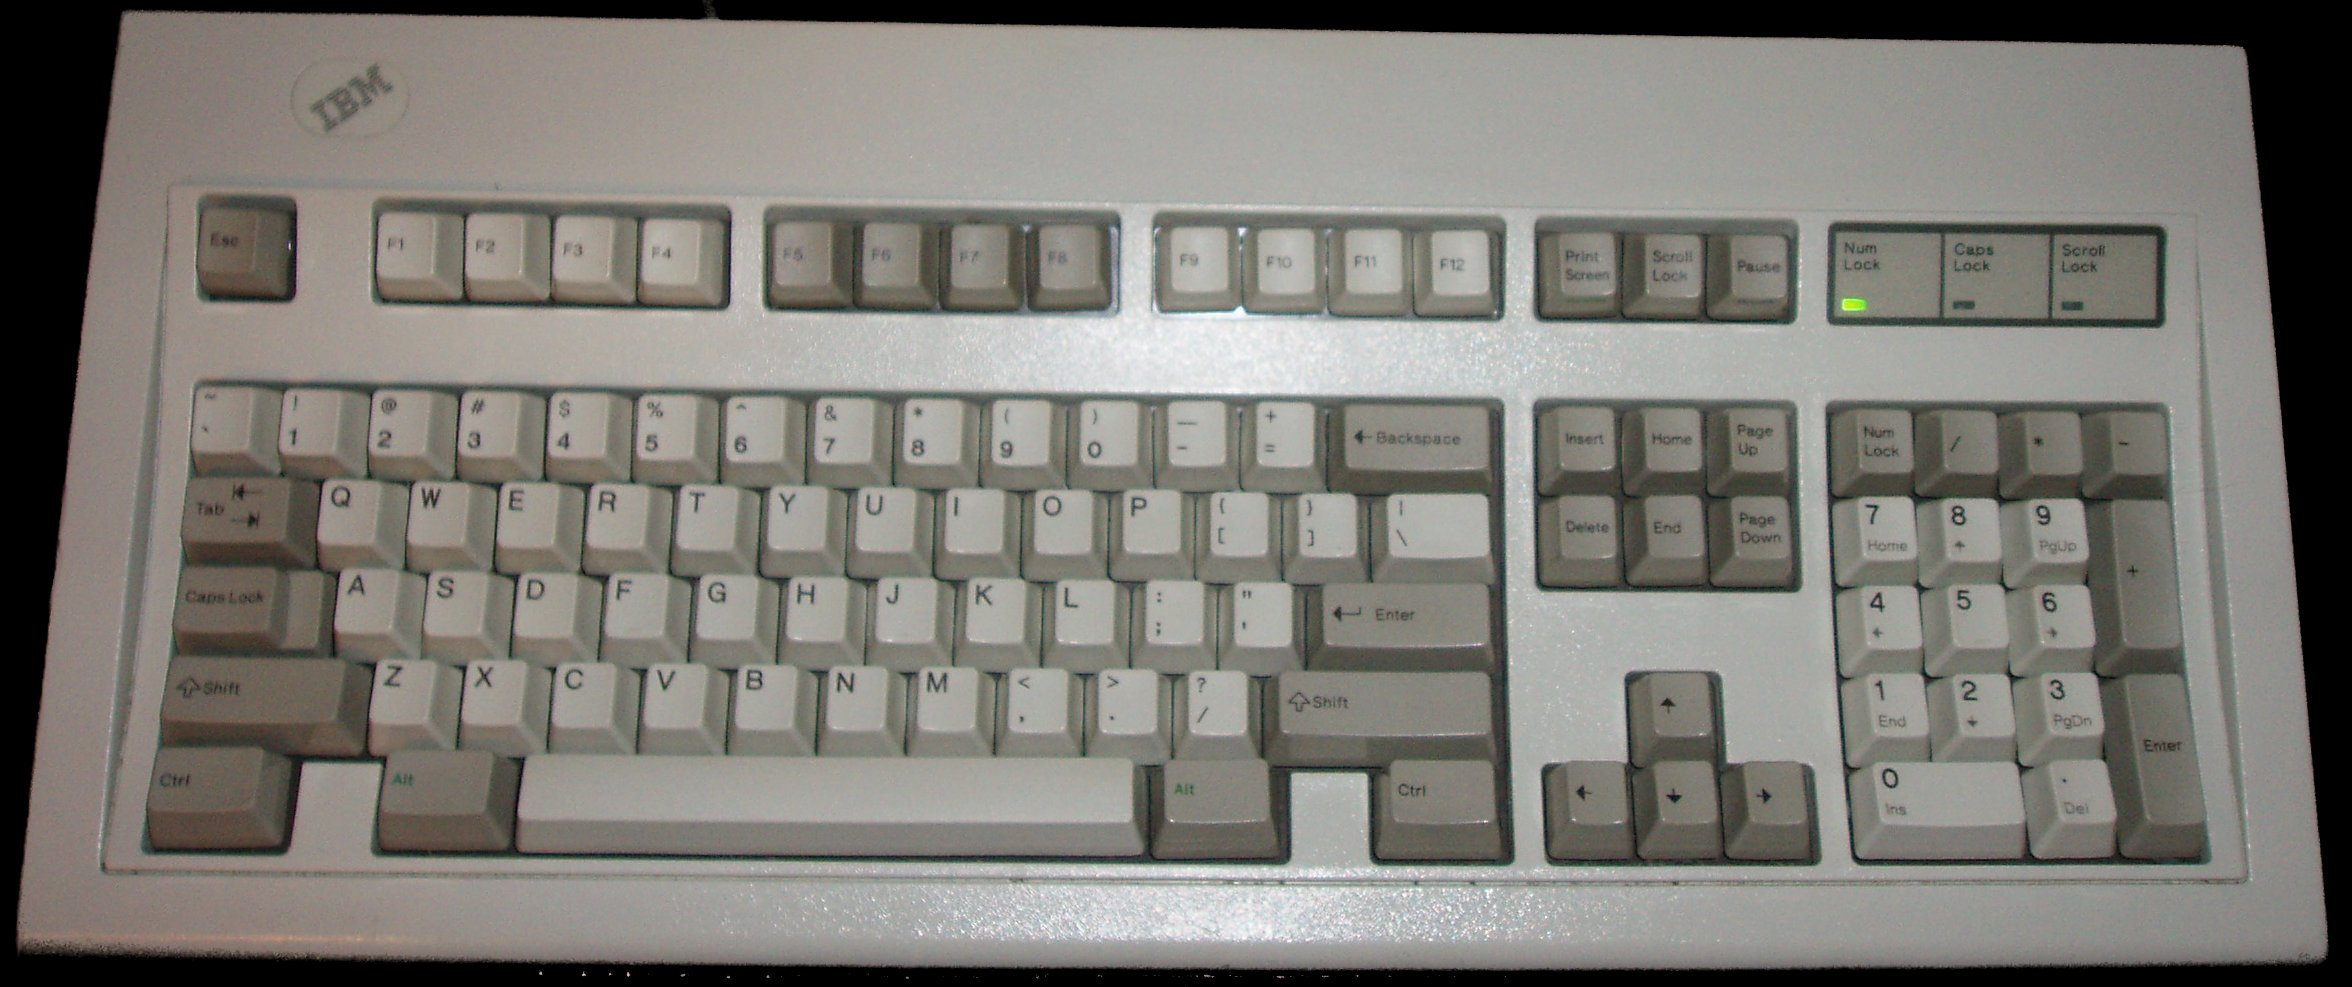
\includegraphics{assets/img/keyboard.jpg}
\end{frame}

\begin{frame}{My first useful program}
\protect\hypertarget{my-first-useful-program}{}
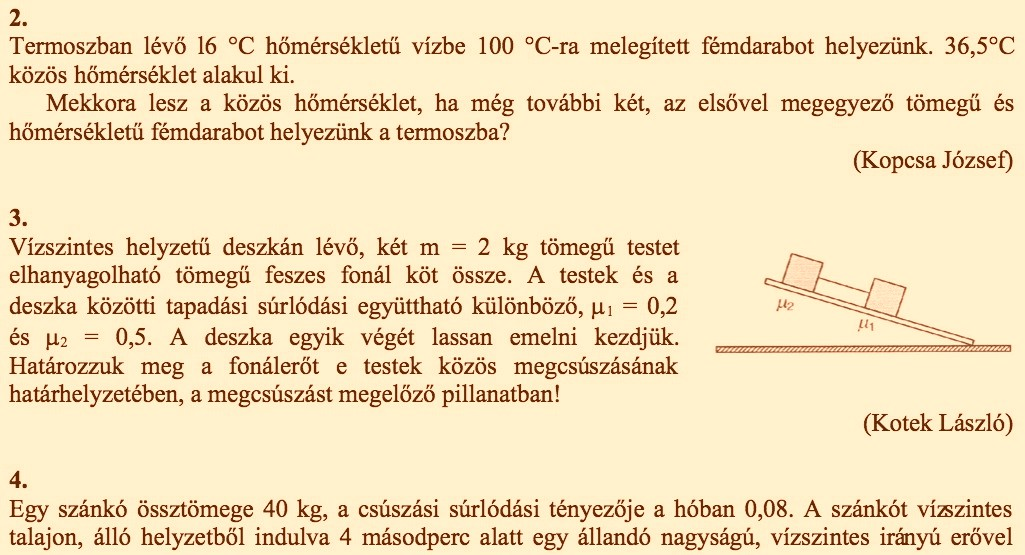
\includegraphics{assets/img/stencil.png}
\end{frame}

\begin{frame}{My first investment in data science}
\protect\hypertarget{my-first-investment-in-data-science}{}
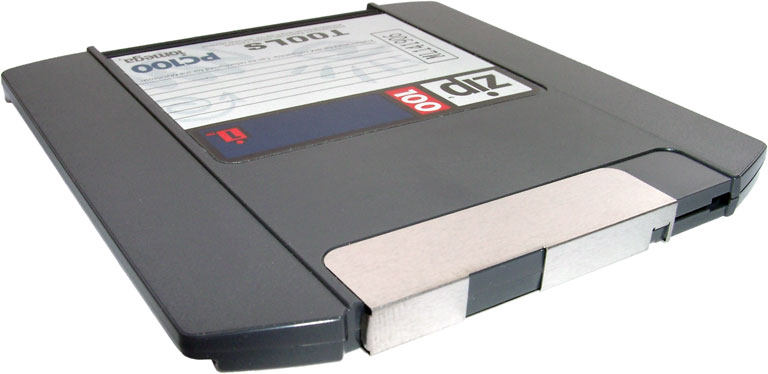
\includegraphics{assets/img/zipdrive.jpg}
\end{frame}

\begin{frame}{My three hats}
\protect\hypertarget{my-three-hats}{}
\begin{enumerate}
\tightlist
\item
  Research
\item
  Teaching
\item
  Reproducibility
\end{enumerate}
\end{frame}

\begin{frame}{Research}
\protect\hypertarget{research}{}
Where: CEU MicroData, KRTK

What: firm and worker behavior in the face of globalization and
technical change. Mostly observational data.
\end{frame}

\begin{frame}{Teaching}
\protect\hypertarget{teaching}{}
Where: CEU, European Economic Association, Carpentries, CodedThinking
\end{frame}

\begin{frame}{Reproducibility}
\protect\hypertarget{reproducibility}{}
Where: Data Editor at Review of Economic Studies (\#5 journal in
economics)

What: Ensure data and code produce results published. Educate authors
about best practices.
\end{frame}

\hypertarget{academic-research}{%
\section{Academic Research}\label{academic-research}}

\begin{frame}{Features of academic research}
\protect\hypertarget{features-of-academic-research}{}
\begin{enumerate}
\tightlist
\item
  Always new questions, always new data
\item
  Often new methods (!)
\item
  Batch processing of ``historical'' data
\item
  Full transparency (!)
\end{enumerate}
\end{frame}

\hypertarget{my-tools}{%
\section{My Tools}\label{my-tools}}

\begin{frame}{The pragmatic programmer}
\protect\hypertarget{the-pragmatic-programmer}{}
\begin{figure}
\centering
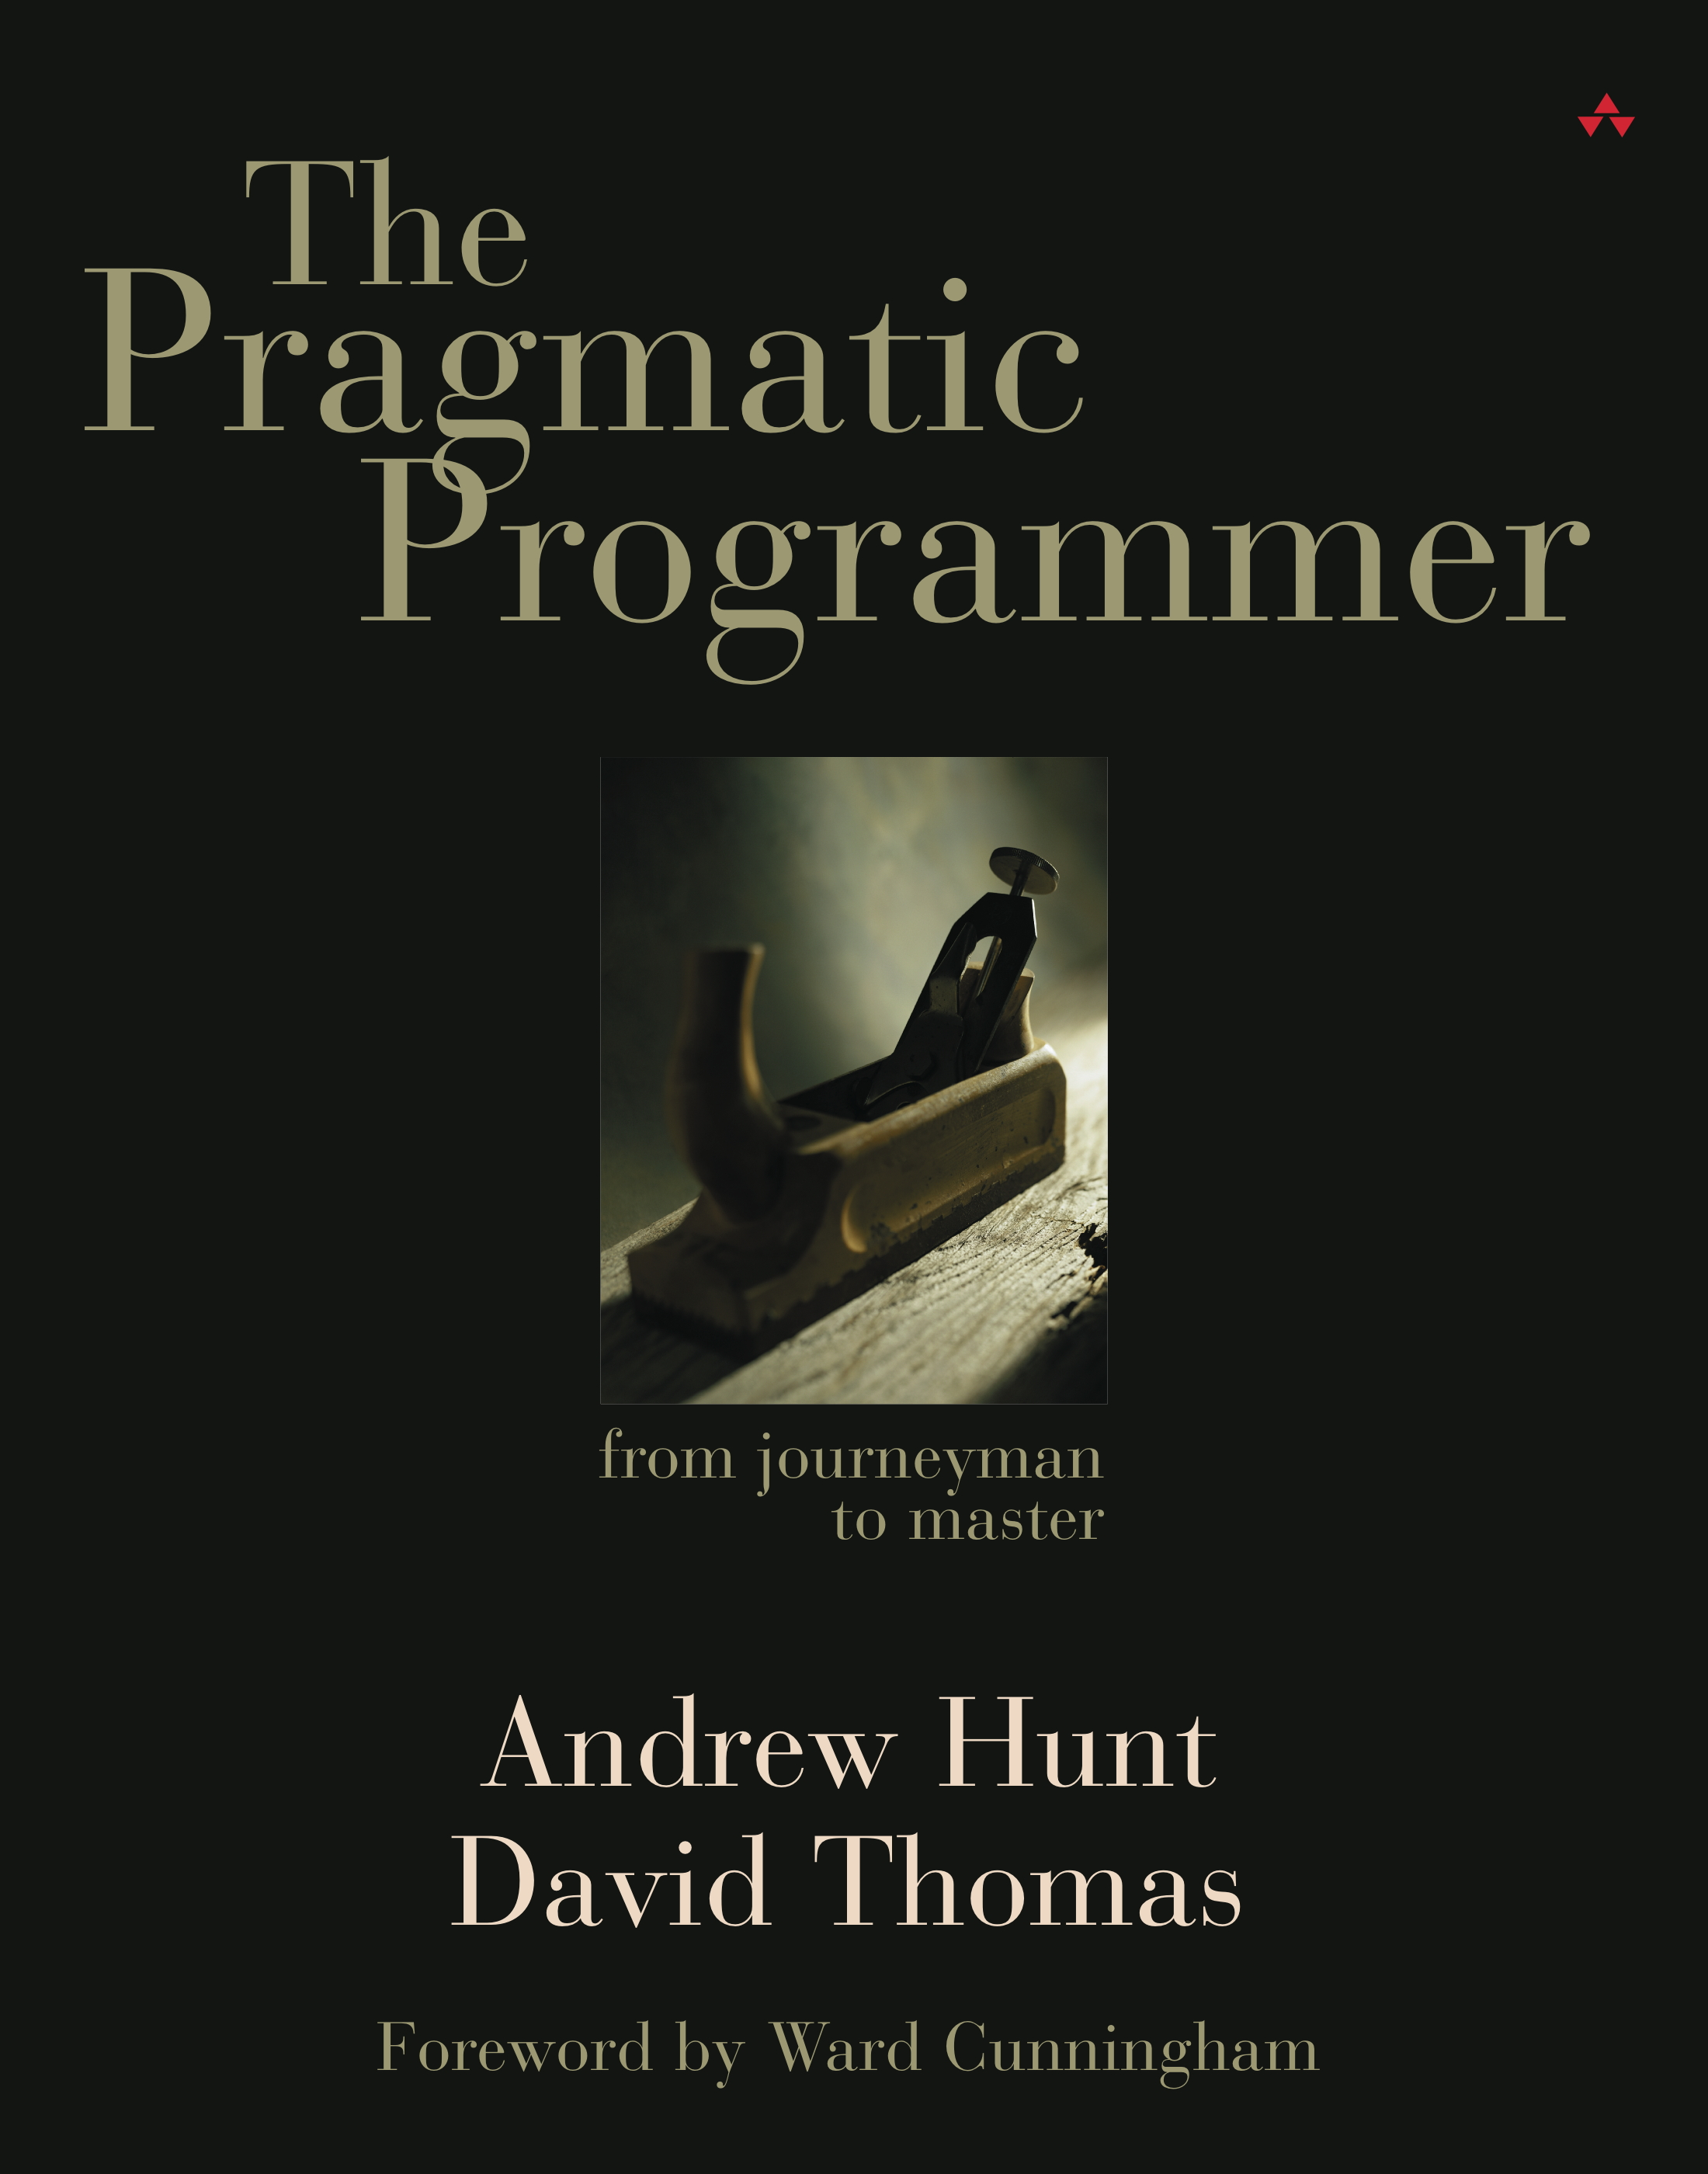
\includegraphics{assets/img/pragmatic.jpg}
\caption{Hunt and Thomas 1999}
\end{figure}
\end{frame}

\begin{frame}{Generic tools and technologies}
\protect\hypertarget{generic-tools-and-technologies}{}
\begin{enumerate}
\tightlist
\item
  Plain text: .csv, .md, .yaml, .tex
\item
  Command line:
\item
  Version control: git, GitHub, Sublime Merge
\item
  Dependency management: Make, bead
\end{enumerate}
\end{frame}

\begin{frame}{Specific tools and technologies}
\protect\hypertarget{specific-tools-and-technologies}{}
\begin{enumerate}
\tightlist
\item
  Data wrangling: Python (not pandas, not .ipynb), Stata
\item
  Statistics: Stata (no R jokes please)
\item
  Simulation: Julia
\end{enumerate}
\end{frame}

\hypertarget{recent-projects}{%
\section{Recent Projects}\label{recent-projects}}

\begin{frame}{Recent projects}
\protect\hypertarget{recent-projects-1}{}
\begin{itemize}
\tightlist
\item
  Business Disruptions from Social Distancing
\item
  Expatriate Managers in International Trade
\item
  Political Favoritism in Public Procurement
\item
  CEU-MTA Business Relations Survey
\end{itemize}
\end{frame}

\hypertarget{live-demo}{%
\section{Live Demo}\label{live-demo}}

\end{document}
